\documentclass[tikz, border=8pt]{standalone}
\usepackage{tikz}
\usetikzlibrary{arrows.meta, positioning, shapes.geometric}

\begin{document}
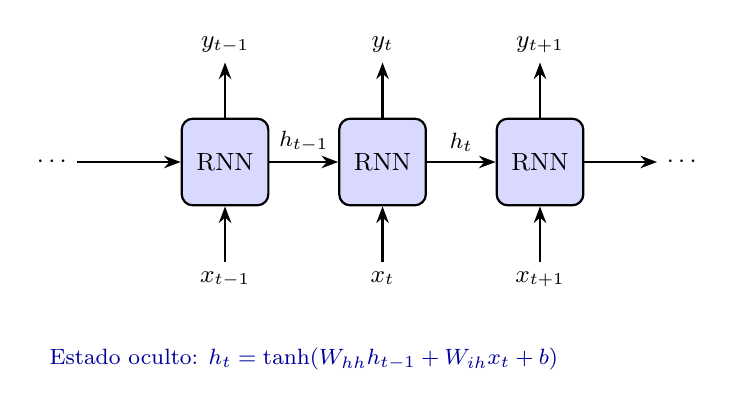
\begin{tikzpicture}[
    cell/.style={draw, rounded corners=4pt, minimum width=1.1cm, minimum height=1.1cm,
                 fill=blue!15, thick},
    arr/.style={-{Stealth[length=6pt]}, thick},
    font=\small
]

% Ellipsis left
\node (ldots) at (-2.2, 0) {$\cdots$};

% Cells
\node[cell] (h0) at (0, 0) {RNN};
\node[above=0.7cm of h0] (y0) {$y_{t-1}$};
\node[below=0.7cm of h0] (x0) {$x_{t-1}$};
\draw[arr] (x0) -- (h0); \draw[arr] (h0) -- (y0);

\node[cell] (h2) at (2, 0) {RNN};
\node[above=0.7cm of h2] (y2) {$y_{t}$};
\node[below=0.7cm of h2] (x2) {$x_{t}$};
\draw[arr] (x2) -- (h2); \draw[arr] (h2) -- (y2);

\node[cell] (h4) at (4, 0) {RNN};
\node[above=0.7cm of h4] (y4) {$y_{t+1}$};
\node[below=0.7cm of h4] (x4) {$x_{t+1}$};
\draw[arr] (x4) -- (h4); \draw[arr] (h4) -- (y4);

% Recurrence arrows
\draw[arr] (ldots) -- (h0);
\draw[arr] (h0) -- node[above, font=\footnotesize]{$h_{t-1}$} (h2);
\draw[arr] (h2) -- node[above, font=\footnotesize]{$h_t$} (h4);

% Ellipsis right
\node (rdots) at (5.8, 0) {$\cdots$};
\draw[arr] (h4) -- (rdots);

% State label
\node[font=\footnotesize, text=blue!60!black] at (1.0, -2.5)
    {Estado oculto: $h_t = \tanh(W_{hh}h_{t-1} + W_{ih}x_t + b)$};

\end{tikzpicture}
\end{document}
